\documentclass[12pt,twoside]{article}
\usepackage[cp1250]{inputenc}
\usepackage[slovene]{babel}
\usepackage[a4paper,width=160mm,height=250mm,left=25mm,right=25mm,top=25mm,bottom=25mm,nohead]{geometry}
\usepackage{graphicx}
\usepackage{times,color}
\usepackage{booktabs}
\usepackage{myijs}
\usepackage[colorlinks,breaklinks,backref,bookmarks]{hyperref}
\usepackage{psfrag}
% USER DEFINED MACROS
\newcommand{\matlab}{MATLAB\textsuperscript{\textregistered}}
\newcommand{\simulink}{SIMULINK\textsuperscript{\textregistered}}
\newcommand{\matsim}{MATLAB\textsuperscript{\textregistered} SIMULINK\textsuperscript{\textregistered}}
\newcommand{\rtsim}{Simulink Real-Time\textsuperscript{\texttrademark}}
\newcommand{\thom}{$\textbf{T}^i_{i+1}$}
\newcommand{\Lagrt}{\mathcal{T}}
\newcommand{\Lagrl}{\mathcal{L}}
\newcommand{\Lagru}{\mathcal{U}}

\usepackage{listings}
\usepackage{color}
\usepackage{textcomp}
\definecolor{listinggray}{gray}{0.9}
\definecolor{lbcolor}{rgb}{0.9,0.9,0.9}
\lstset{
	backgroundcolor=\color{lbcolor},
	tabsize=4,
	rulecolor=,
	language=C++,
        basicstyle=\scriptsize,
        upquote=true,
        aboveskip={1.5\baselineskip},
        columns=fixed,
        showstringspaces=false,
        extendedchars=true,
        breaklines=true,
        prebreak = \raisebox{0ex}[0ex][0ex]{\ensuremath{\hookleftarrow}},
        frame=single,
        showtabs=false,
        showspaces=false,
        showstringspaces=false,
        identifierstyle=\ttfamily,
        keywordstyle=\color[rgb]{0,0,1},
        commentstyle=\color[rgb]{0.133,0.545,0.133},
        stringstyle=\color[rgb]{0.627,0.126,0.941},
				numbers=left,                   % where to put the line-numbers
				numberstyle=\footnotesize,      % the size of the fonts that are used for the line-numbers
				stepnumber=2,                   % the step between two line-numbers. If it's 1 each line will be numbered
				numbersep=5pt,
}





\parindent 0cm
\parskip 0.5\baselineskip
\renewcommand{\topfraction}{.99}
\renewcommand{\bottomfraction}{.99}
\renewcommand{\textfraction}{.01}
\renewcommand{\floatpagefraction}{.99}



\renewcommand{\topfraction}{.99}
\renewcommand{\bottomfraction}{.99}
\renewcommand{\textfraction}{.01}
\renewcommand{\floatpagefraction}{.99}

 \newcommand{\mhs}{\hspace{0.5cm}}
 \newcommand{\mds}{\displaystyle}

 \font\titlefonta= phvb at 35pt
 \font\titlefontb= cmbx12 at 70pt



\hypersetup{pdftitle=udp-arcnet,pdfauthor=Timotej Ga�par,
            pdfsubject=Control of PA-10 robot via UDP-ARCNET server,
            pdfkeywords=}

\begin{document}
\null \vspace{1.5cm}

\IJSglava

 \null\hfill{\sffamily DP 10322}

\vspace{2cm}

\vspace{2cm}


\null\hfill{\LARGE \sffamily \textbf{Control of PA-10 robot via UDP-ARCNET server}}


\vspace{1cm}

\null\hfill{\large \slshape Timotej Ga�par, Leon �lajpah}

\vfill

%\centerline{\includegraphics[height=8cm]{figures/Logo_pic.eps}}

\vfill



\centerline{\sffamily Ljubljana, oktober 2015}

%\newpage
%\null

\newpage
\tableofcontents

\normalsize

\newpage



\section{Introduction}\

The report presents a server developed for the purpose of controlling the robot Mitsubishi PA-10 via Ethernet by sending UDP packets. The server acts as middleware between the UDP client and the ARCNET robot controller of the servomotors of the PA-10 robot. It works in real time with a sample frequency of 500Hz. It also allows to control the robot through the internal speed or torque regulator, which gives the users freedom to implement various control strategies.

The thesis presents the use of various robot control strategies. Experiments with velocity and torque control modes have been made in joint and task space.  Additional experiments also showed the possibility to control the robot in contact with the environment. The results of the experiments showed that the velocity control works better as it is not as dependent on the robot's dynamic parameters as the torque control mode which was implemented with the use of the dynamic model. But due to the probably imprecise dynamic model parameters used for the realization of the different torque mode controls the results of these are not as satisfactory.

Higher level control was developed in \matsim programme. We developed a \simulink block for communication with the developed server which gives future users easier ways to implement control algorithms.
	
%The robot Mitsubishi Portable Arm PA-10 is a serial robot with seven degrees of freedom. It's servo motor controller allows control of the robot via input speeds or input torques. The controller has an ARCNET module which allows its connection to the ARCNET network. We developed a UDP-ARNCET server program, to allow future users to develop various control programs without the need to directly connect to the robot's servo controller. The only requisite is the ability of the control program to send UDP packages to the UDP-ARCNET server.
%
%Matlab's Simulink Real-Time OS offers the ability to develop programs that run in hard real time. We implemented various control strategies that control the robot via input speeds or input torques. For easier start we also prepared basic control schemes which are easily accessible from the Matlab's command line.


\begin{figure}
	\begin{center}
		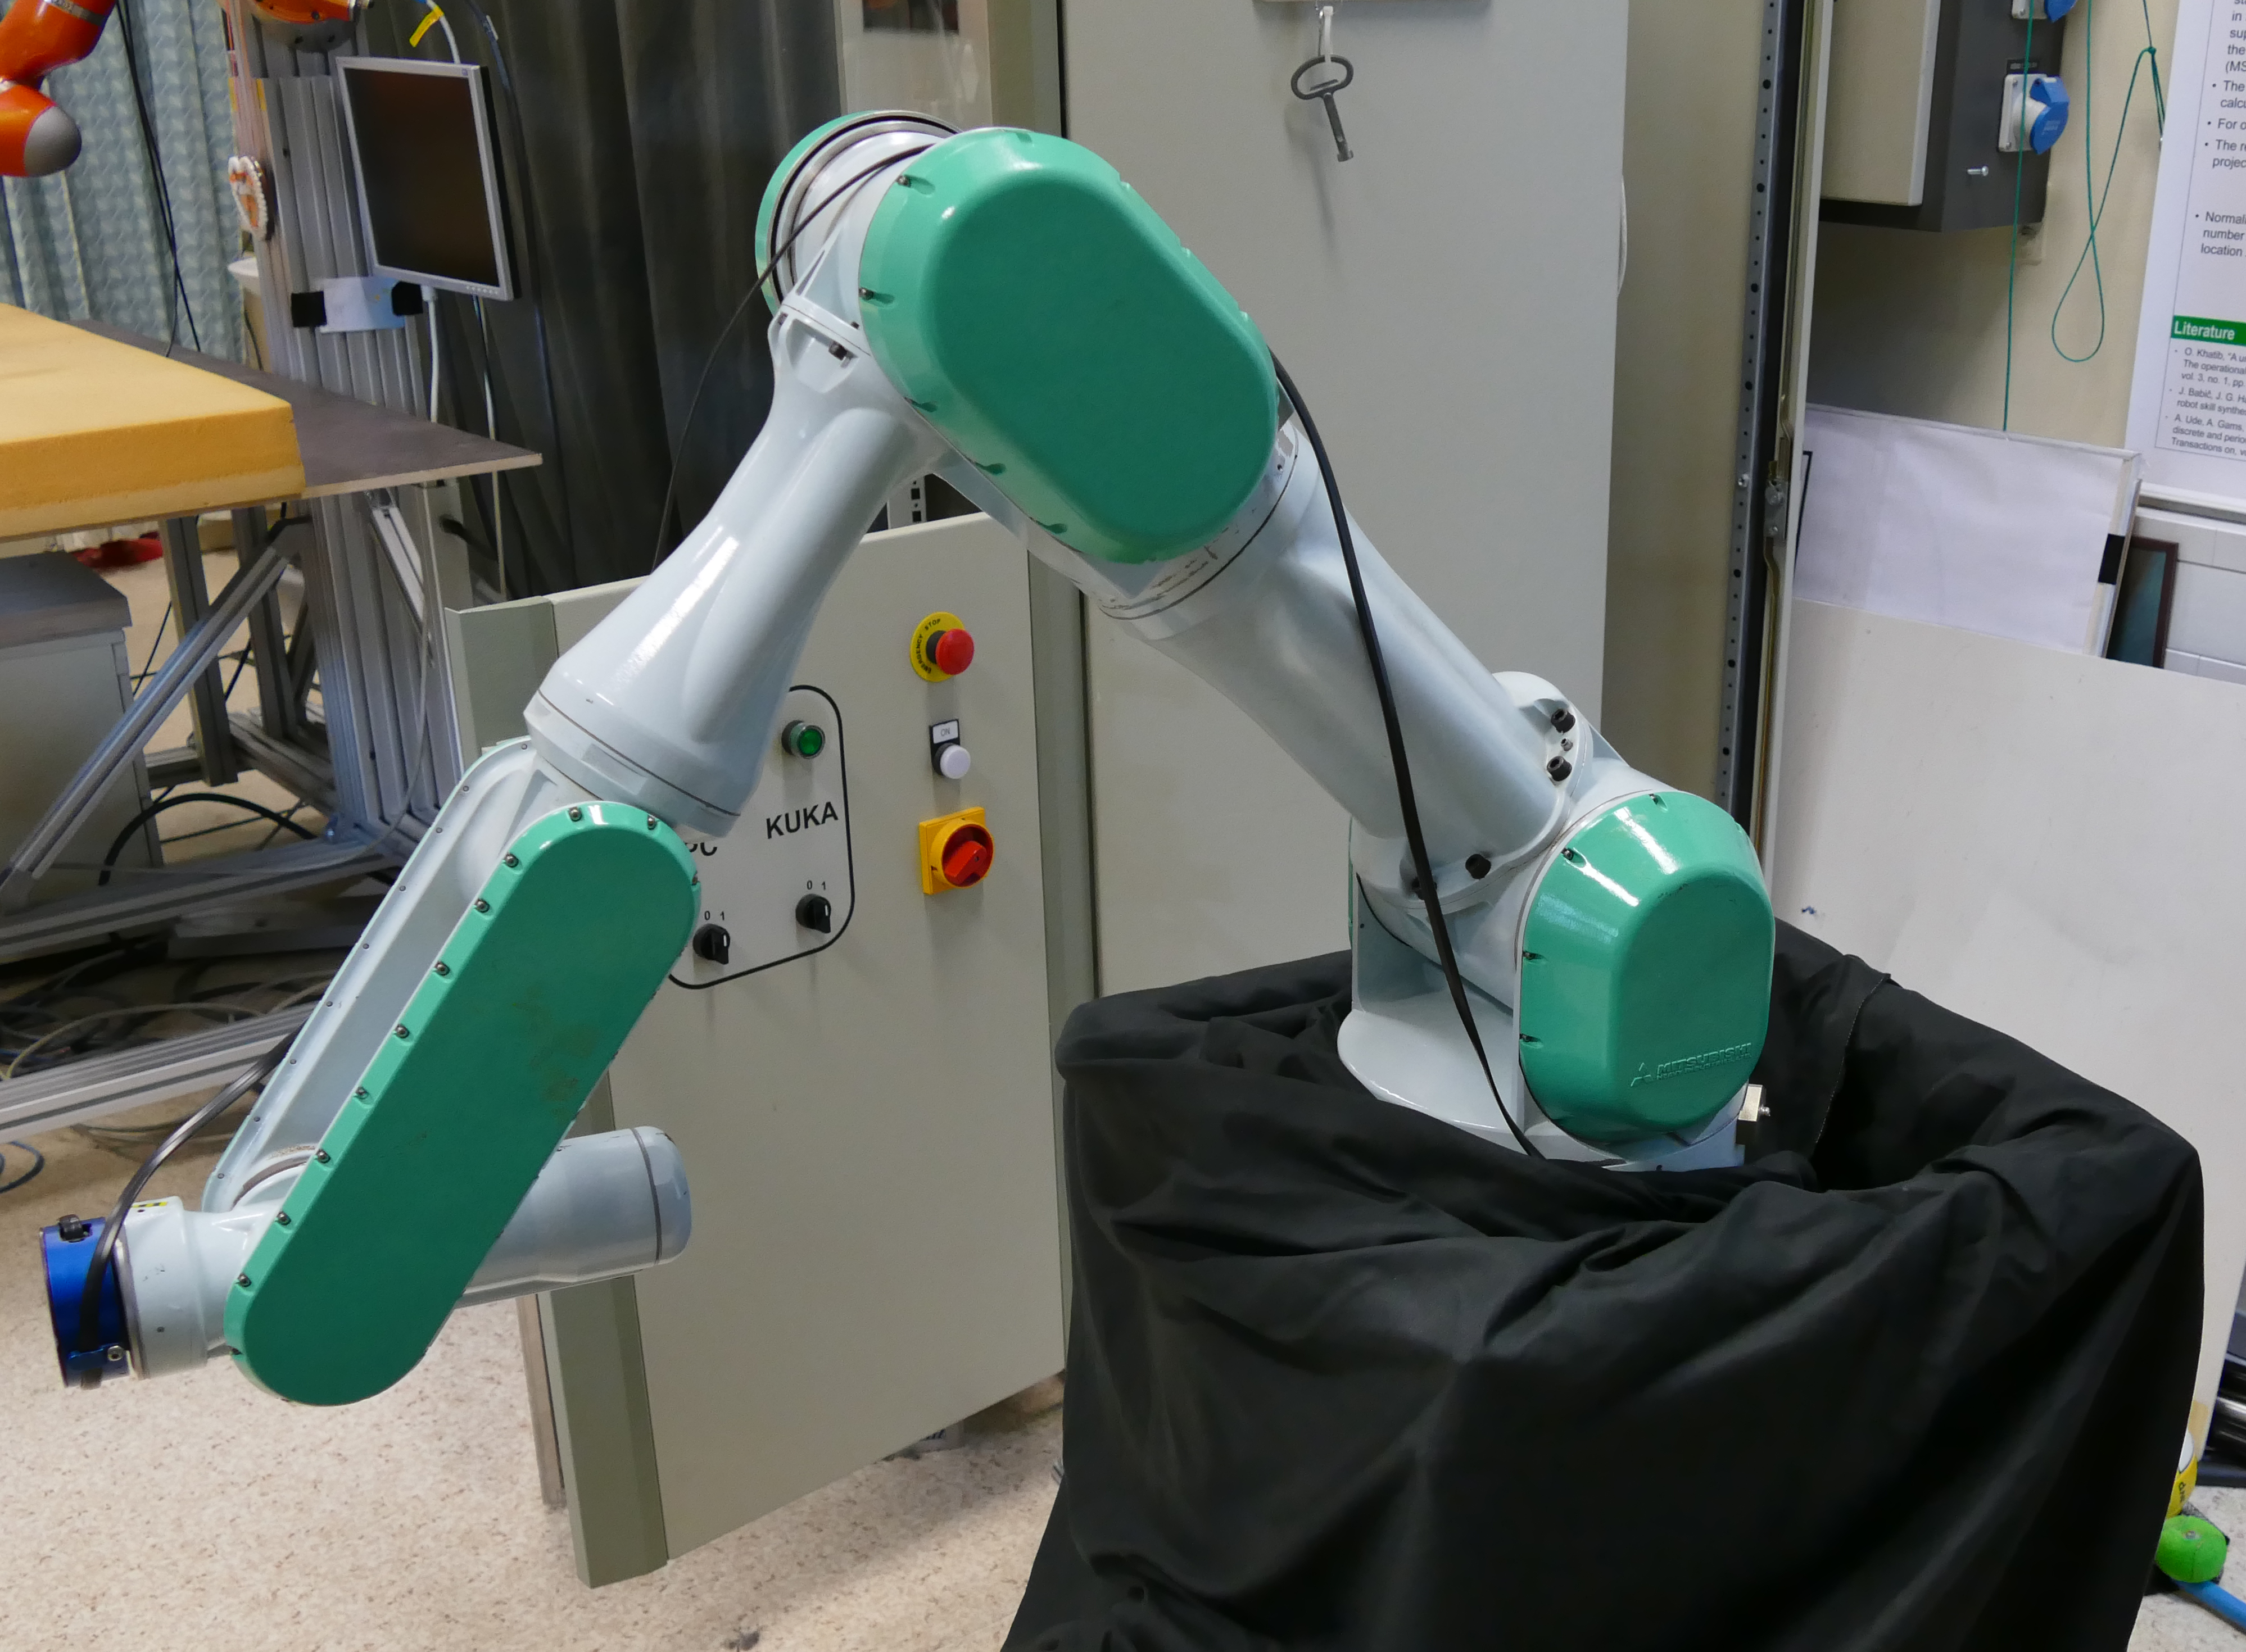
\includegraphics[scale=0.2]{./slike/pa10.png}
		\caption{Mitsubishi Portable Arm PA-10 robot.} \label{slika}
		\end{center}
\end{figure}

\section{UDP-ARCNET server}
\subsection{Specifications}
\subsection{Usage}
\subsection{Modding}


\section{Simulink Real-Time client}
\


\section{Literatura}

\end{document}




